% Task 9: is the keystream uniform? CHECKED with python3 and Task9/rc4.py:
%   random.seed(9), keys of 16 random bytes, z = prga(ksa(key), 3); picked: five keys without a 0,
%   one with z[0] = 0, one with z[2] = 0 (so that the example does not point at byte 2):
%   6ea68776... 10 bf a8 | aa517723... ca bc 7a | 21b1479c... 00 76 36 | 50baa501... 09 ac bc
%   1ddbf6e5... 35 28 12 | 7ff75213... 0a fd 00 | 47abe48d... 91 e5 a7
%   1/256 = 0.39%. The measured percentages are the result of the task: not shown.
\documentclass[12pt,tikz,border=6pt]{standalone}
% Shared preamble of the task figures of Lecture 1.
% The colours and styles are copied from the preamble of ../main.tex (keep them in sync).
\usepackage{lmodern}
\usepackage[T1]{fontenc}
\renewcommand{\familydefault}{\sfdefault}
\usepackage{amsmath,amssymb}
\usepackage{xcolor}
\usepackage{fontawesome5}
\usetikzlibrary{arrows.meta, calc, positioning, fit, decorations.pathreplacing, decorations.pathmorphing, backgrounds}

% ---------- template ----------
\definecolor{DeepBlue}{HTML}{283593}
\definecolor{AccentOrange}{HTML}{EB5A14}
\definecolor{LightGray}{HTML}{F5F6FA}
% ---------- actors and categories (S1 to S6) ----------
\definecolor{sIndigo}{HTML}{5C6BC0}   % the sender
\definecolor{sPink}{HTML}{EC407A}     % the attacker
\definecolor{sViolet}{HTML}{7E57C2}   % plaintext
\definecolor{sAmber}{HTML}{FFB300}    % key and keystream
\definecolor{sTeal}{HTML}{26A69A}     % the receiver
\definecolor{sBrown}{HTML}{8D6E63}    % ciphertext
\definecolor{sPinkText}{HTML}{C2185B}
\definecolor{sAmberText}{HTML}{A06A00}
\definecolor{sTealText}{HTML}{00796B}
% ---------- actions and results ----------
\definecolor{aExec}{HTML}{43A047}
\definecolor{aRead}{HTML}{1E88E5}
\definecolor{aWrite}{HTML}{E53935}
% ---------- neutral ----------
\definecolor{nInk}{HTML}{37474F}
\definecolor{nLine}{HTML}{90A4AE}
\definecolor{nLight}{HTML}{CFD8DC}
\definecolor{nFill}{HTML}{ECEFF1}
\definecolor{nIdle}{HTML}{E0E0E0}

% ---------- TikZ styles (as in main.tex; byte cells a little larger for the web) ----------
\tikzset{
  hw/.style={draw=nLine, thick, fill=nFill, text=nInk, rounded corners=3pt, align=center, inner sep=4pt},
  hwmain/.style={draw=nInk, thick, fill=nInk, text=white, rounded corners=3pt, align=center, inner sep=4pt},
  cell/.style={draw=nLine, thick, fill=white, text=nInk, font=\ttfamily\small},
  cellfree/.style={cell, dashed, draw=nLight},
  container/.style={draw=nLine, thick, dashed, rounded corners=5pt},
  actor/.style={fill=#1, draw=#1, text=white, rounded corners=3pt, align=center, font=\small\bfseries, inner sep=5pt},
  actorlight/.style={fill=#1!15, draw=#1, thick, text=nInk, rounded corners=3pt, align=center, inner sep=5pt},
  data/.style={-{Stealth}, very thick, nInk},
  flow/.style={-{Stealth}, very thick, DeepBlue},
  annot/.style={draw=AccentOrange, line width=1.6pt, rounded corners=3pt},
  byte/.style={draw=nLine, thick, fill=white, text=nInk, font=\ttfamily\small,
    minimum width=0.8cm, minimum height=0.62cm, inner sep=1pt, rounded corners=1.5pt},
  ptb/.style={byte, fill=sViolet!15, draw=sViolet},
  ksb/.style={byte, fill=sAmber!25, draw=sAmber},
  ctb/.style={byte, fill=sBrown!15, draw=sBrown},
  unk/.style={byte, fill=white, dashed, text=sViolet},
  rowlabel/.style={font=\small\bfseries, text=nInk, anchor=east},
  note/.style={font=\small, text=nInk},
  bigxor/.style={circle, draw=nInk, very thick, fill=white, inner sep=0pt, minimum size=0.8cm, font=\Large},
  radio/.style={-{Stealth}, very thick, nInk, decorate,
    decoration={snake, amplitude=1.2pt, segment length=7pt, post length=4pt}},
  % a white card behind the whole figure, so that it stays readable in a dark theme
  card/.style={show background rectangle, background rectangle/.style={fill=white, draw=none}, inner frame sep=8pt},
}
% a row of bytes: \byterow{x of the first cell}{y}{style}{list of values}{step between cells}
\newcommand{\byterow}[5]{%
  \expandafter\def\expandafter\brlist\expandafter{#4}%
  \foreach \v [count=\k from 0] in \brlist {
    \node[#3] at ({#1+#5*\k},#2) {\v};
  }}
% the generator / cipher box: dark, with cogs. \cogbox{name}{position}{label}{width}
\newcommand{\cogbox}[4]{%
  \node[hwmain, minimum width=#4, minimum height=1.3cm] (#1) at (#2) {};
  \node[text=white, font=\Large] at ([yshift=0.22cm]#1.center) {\faCogs};
  \node[text=white, font=\small\bfseries] at ([yshift=-0.32cm]#1.center) {#3};}
\newcommand{\ok}{\textcolor{aExec}{\faCheck}}
\newcommand{\nok}{\textcolor{aWrite}{\faTimes}}
\newcommand{\badge}[1]{\tikz[baseline=(b.base)]\node[circle,fill=AccentOrange,text=white,
  inner sep=1.5pt,font=\bfseries\footnotesize] (b) {#1};}

\begin{document}
\pagecolor{white}
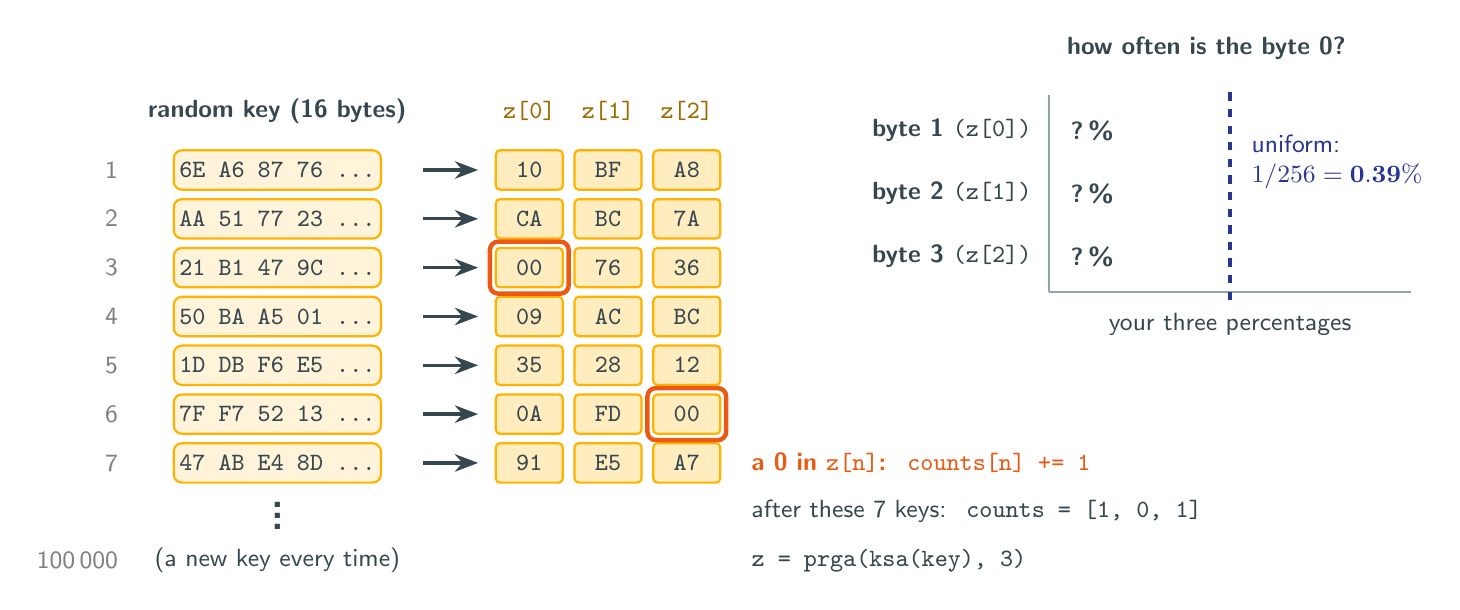
\begin{tikzpicture}[>=Stealth]
  \def\dy{0.62}
  \tikzset{zb/.style={ksb, minimum width=0.85cm, minimum height=0.5cm}}
  % the table of keys and their first 3 keystream bytes
  \node[font=\small\bfseries, text=nInk] at (1.8,0.75) {random key (16 bytes)};
  \foreach \c/\l in {0/{z[0]},1/{z[1]},2/{z[2]}} \node[font=\ttfamily\small\bfseries, text=sAmberText] at ({5.0+1.0*\c},0.75) {\l};
  \foreach \k/\key/\z [count=\r from 0] in {1/{6E A6 87 76 \ldots}/{10,BF,A8}, 2/{AA 51 77 23 \ldots}/{CA,BC,7A},
      3/{21 B1 47 9C \ldots}/{00,76,36}, 4/{50 BA A5 01 \ldots}/{09,AC,BC}, 5/{1D DB F6 E5 \ldots}/{35,28,12},
      6/{7F F7 52 13 \ldots}/{0A,FD,00}, 7/{47 AB E4 8D \ldots}/{91,E5,A7}} {
    \node[font=\small, text=gray, anchor=east] at (-0.1,{-\dy*\r}) {\k};
    \node[actorlight=sAmber, font=\ttfamily\small, minimum height=0.5cm, inner sep=2pt] at (1.8,{-\dy*\r}) {\key};
    \draw[data] (3.65,{-\dy*\r}) -- (4.35,{-\dy*\r});
    \byterow{5.0}{-\dy*\r}{zb}{\z}{1.0}
  }
  \node[font=\Large\bfseries, text=nInk] at (1.8,{-\dy*7+0.05}) {$\vdots$};
  \node[font=\small, text=gray, anchor=east] at (-0.1,{-\dy*8}) {100\,000};
  \node[font=\small, text=nInk] at (1.8,{-\dy*8}) {(a new key every time)};
  \draw[annot] (4.5,{-\dy*2-0.33}) rectangle (5.5,{-\dy*2+0.33});
  \draw[annot] (6.5,{-\dy*5-0.33}) rectangle (7.5,{-\dy*5+0.33});
  \node[font=\small\bfseries, text=AccentOrange, anchor=west] at (7.7,{-\dy*6}) {a 0 in \texttt{z[n]}: \ \texttt{counts[n] += 1}};
  \node[font=\small, text=nInk, anchor=west] at (7.7,{-\dy*7}) {after these 7 keys: \ \texttt{counts = [1, 0, 1]}};
  \node[font=\small, text=nInk, anchor=west] at (7.7,{-\dy*8}) {\ttfamily z = prga(ksa(key), 3)};

  % the idea: compare each percentage with the uniform line
  \begin{scope}[shift={(11.6,-1.2)}]
    \node[font=\small\bfseries, text=nInk] at (2.0,2.75) {how often is the byte 0?};
    \draw[nLine, thick] (0,-0.35) -- (0,2.15);
    \draw[nLine, thick] (0,-0.35) -- (4.6,-0.35);
    \foreach \l/\y in {{byte 1 \texttt{(z[0])}}/1.7, {byte 2 \texttt{(z[1])}}/0.9, {byte 3 \texttt{(z[2])}}/0.1} {
      \node[font=\small\bfseries, text=nInk, anchor=east] at (-0.1,\y) {\l};
      \node[font=\small\bfseries, text=nInk, anchor=west] at (0.15,\y) {?\,\%};
    }
    \draw[DeepBlue, very thick, dashed] (2.3,-0.45) -- (2.3,2.25);
    \node[font=\small, text=DeepBlue, anchor=west, align=left] at (2.45,1.3) {uniform:\\ $1/256 = \mathbf{0.39\%}$};
    \node[font=\small, text=nInk, anchor=north, align=center] at (2.3,-0.5) {your three percentages};
  \end{scope}
\end{tikzpicture}
\end{document}
